\documentclass[twocolumn,10pt]{article}
\title{Benchmark angles}
\setlength{\columnsep}{20pt} 
\usepackage{amsmath,hyperref,cancel,graphicx}
 \def\shrinkfactor{0.55}
 \usepackage[margin=1.5cm]{geometry}
\usepackage[usenames,dvipsnames]{color}
 
 \newcommand{\blue}[1]{{\color{Blue}#1}} 
 \newcommand{\purple}[1]{{\color{Purple}#1}} 
 \newcommand{\red}[1]{{\color{Red}#1}} 
 \newcommand{\green}[1]{{\color{Green}#1}} 
 \newcommand{\gray}[1]{{\color{Gray}#1}} 
  \newcommand{\pink}[1]{{\color{Magenta}#1}}   


\begin{document}
\maketitle



\section{\href{https://www.khanacademy.org/devadmin/content/items/x3554cca2a4f26df7}{x3554cca2a4f26df7}}

\noindent
**Which of these angles has a measure of 90�?**

\paragraph{Ans} 


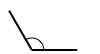
\includegraphics[scale=\shrinkfactor]{figures/30e6d029e2da9ba1853a868eb2f393092111abdd.png}



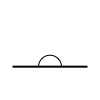
\includegraphics[scale=\shrinkfactor]{figures/567e8914a4f3bc1f9bca20b50f74d304dad89471.png}


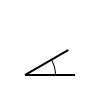
\includegraphics[scale=\shrinkfactor]{figures/d3a2a4fb2274b18d8b340c80127ae99c1ed8b1f9.png}

\fbox{ 
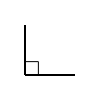
\includegraphics[scale=\shrinkfactor]{figures/e6ad77b54552295693aae7e39624ed456b552099.png}

}

 

\paragraph{Hint 1}We can easily identify a $90^\circ$ angle.  It looks like the corner of a rectangular piece of paper or a door.  Sometimes, it is marked with a little square inside of the angle.

\paragraph{Hint 2}This angle is a $90^\circ$ angle.  


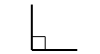
\includegraphics[scale=\shrinkfactor]{figures/59dcaf7caad1b34a49fc6b67de97830d5c26786c.png}



\medskip
\noindent
\textbf{Tags:} {\footnotesize CC.4.MD.C.5, SB.4.1.K.4.SR, Benchmark angles.1, Benchmark angles}\\
\textbf{Version:} 8f650d3f.. 2013-10-11
\smallskip\hrule





\section{\href{https://www.khanacademy.org/devadmin/content/items/x42f174ad068a99ce}{x42f174ad068a99ce}}

\noindent
**Which of these angles has a measure of 60�?**

\paragraph{Ans} 


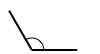
\includegraphics[scale=\shrinkfactor]{figures/30e6d029e2da9ba1853a868eb2f393092111abdd.png}



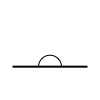
\includegraphics[scale=\shrinkfactor]{figures/567e8914a4f3bc1f9bca20b50f74d304dad89471.png}


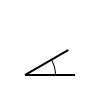
\includegraphics[scale=\shrinkfactor]{figures/d3a2a4fb2274b18d8b340c80127ae99c1ed8b1f9.png}

\fbox{ 
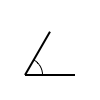
\includegraphics[scale=\shrinkfactor]{figures/a78f141720cba4a3b167228345493573d23a2d23.png}

}

 

\paragraph{Hint 1}The $60^\circ$ angle will have to be acute, which means smaller than a $90^\circ$ angle.  Two of the answer choices are acute angles.


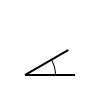
\includegraphics[scale=\shrinkfactor]{figures/d3a2a4fb2274b18d8b340c80127ae99c1ed8b1f9.png}

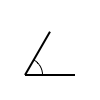
\includegraphics[scale=\shrinkfactor]{figures/a78f141720cba4a3b167228345493573d23a2d23.png}

\paragraph{Hint 2}A $60^\circ$ angle is $\frac{2}{3}$ the size of a $90^\circ$ angle.  That means that it is more than half the size of a $90^\circ$ angle.

Which angle looks bigger than half of a $90^\circ$ angle?

\paragraph{Hint 3}Here is a $90^\circ$ angle cut into a $60^\circ$ angle and a $30^\circ$ angle.  

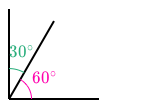
\includegraphics[scale=\shrinkfactor]{figures/8eb18621606206c7adf43aa4f147027fdea82fad.png}

\paragraph{Hint 4}This angle is a $60^\circ$ angle.  

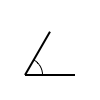
\includegraphics[scale=\shrinkfactor]{figures/a78f141720cba4a3b167228345493573d23a2d23.png}



\medskip
\noindent
\textbf{Tags:} {\footnotesize CC.4.MD.C.5, SB.4.1.K.4.SR, Benchmark angles.1, Benchmark angles}\\
\textbf{Version:} b3113463.. 2013-10-11
\smallskip\hrule





\section{\href{https://www.khanacademy.org/devadmin/content/items/x5a53a7885cc1e412}{x5a53a7885cc1e412}}

\noindent
**Which of these angles has a measure of 30�?**

\paragraph{Ans} 


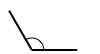
\includegraphics[scale=\shrinkfactor]{figures/30e6d029e2da9ba1853a868eb2f393092111abdd.png}



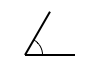
\includegraphics[scale=\shrinkfactor]{figures/fabb944602f99b6fe0a5d55e7d841f87d0cbb415.png}


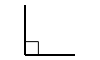
\includegraphics[scale=\shrinkfactor]{figures/07bf5a33ab5404dda360187045fc484bafcf6406.png}

\fbox{ 
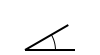
\includegraphics[scale=\shrinkfactor]{figures/5a8d12cf1b68c217e145c1ab706ff0ac470bb360.png}

}

 

\paragraph{Hint 1}We can most easily identify a $90^\circ$ angle.  It looks like the corner of a rectangular piece of paper or a door.  


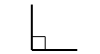
\includegraphics[scale=\shrinkfactor]{figures/59dcaf7caad1b34a49fc6b67de97830d5c26786c.png}

The $30^\circ$ angle will have to be smaller than that one.  Two of the remaining angles are smaller than $90^\circ$.  

\paragraph{Hint 2}A $30^\circ$ angle is $\frac{1}{3}$ the size of a $90^\circ$ angle.  

It takes three $30^\circ$ angles sitting side by side to make one $90^\circ$ angle.  Which angle could you fit $3$ times inside of a $90^\circ$ angle?

\paragraph{Hint 3}Here is a $90^\circ$ angle cut into $3$ angles of $30^\circ$.  


\includegraphics[scale=\shrinkfactor]{figures/32e70b8ce2cad5546c56f4c5d1a1f283fdc91895.png}

\paragraph{Hint 4}The smallest angle pictured is a $30^\circ$ angle.  

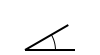
\includegraphics[scale=\shrinkfactor]{figures/5a8d12cf1b68c217e145c1ab706ff0ac470bb360.png}



\medskip
\noindent
\textbf{Tags:} {\footnotesize CC.4.MD.C.5, SB.4.1.K.4.SR, Benchmark angles.1, Benchmark angles}\\
\textbf{Version:} b213797d.. 2013-10-11
\smallskip\hrule





\section{\href{https://www.khanacademy.org/devadmin/content/items/x62d7b969bbdb037a}{x62d7b969bbdb037a}}

\noindent
**Which of these angles has a measure of 135�?**

\paragraph{Ans} 

\fbox{ 
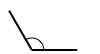
\includegraphics[scale=\shrinkfactor]{figures/30e6d029e2da9ba1853a868eb2f393092111abdd.png}


}

 
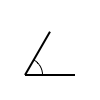
\includegraphics[scale=\shrinkfactor]{figures/a78f141720cba4a3b167228345493573d23a2d23.png}


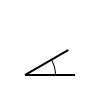
\includegraphics[scale=\shrinkfactor]{figures/d3a2a4fb2274b18d8b340c80127ae99c1ed8b1f9.png}


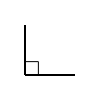
\includegraphics[scale=\shrinkfactor]{figures/e6ad77b54552295693aae7e39624ed456b552099.png}



\paragraph{Hint 1}We can easily identify a $90^\circ$ angle.  It looks like the corner of a rectangular piece of paper or a door.  


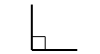
\includegraphics[scale=\shrinkfactor]{figures/59dcaf7caad1b34a49fc6b67de97830d5c26786c.png}

\paragraph{Hint 2}The $135^\circ$ angle will have to be obtuse, which means larger than a $90^\circ$ angle.  Only one of the answer choices is an obtuse angle.

\paragraph{Hint 3}This angle is a $135^\circ$ angle.  


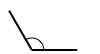
\includegraphics[scale=\shrinkfactor]{figures/30e6d029e2da9ba1853a868eb2f393092111abdd.png}



\medskip
\noindent
\textbf{Tags:} {\footnotesize CC.4.MD.C.5, SB.4.1.K.4.SR, Benchmark angles.1, Benchmark angles}\\
\textbf{Version:} f8eac6aa.. 2013-10-11
\smallskip\hrule





\section{\href{https://www.khanacademy.org/devadmin/content/items/x8ee189a99eeb0414}{x8ee189a99eeb0414}}

\noindent
**Which of these angles has a measure of 180�?**

\paragraph{Ans} 

\fbox{ 
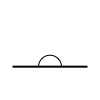
\includegraphics[scale=\shrinkfactor]{figures/567e8914a4f3bc1f9bca20b50f74d304dad89471.png}


}

 
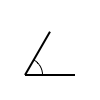
\includegraphics[scale=\shrinkfactor]{figures/a78f141720cba4a3b167228345493573d23a2d23.png}


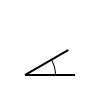
\includegraphics[scale=\shrinkfactor]{figures/d3a2a4fb2274b18d8b340c80127ae99c1ed8b1f9.png}


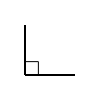
\includegraphics[scale=\shrinkfactor]{figures/e6ad77b54552295693aae7e39624ed456b552099.png}



\paragraph{Hint 1}A $180^\circ$ angle is a special angle called a *straight angle*.  This means that the two sides of the angle stretch out to form a straight line.

\paragraph{Hint 2}This angle is a $180^\circ$ angle.  


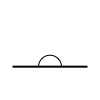
\includegraphics[scale=\shrinkfactor]{figures/567e8914a4f3bc1f9bca20b50f74d304dad89471.png}



\medskip
\noindent
\textbf{Tags:} {\footnotesize CC.4.MD.C.5, SB.4.1.K.4.SR, Benchmark angles.1, Benchmark angles}\\
\textbf{Version:} 7f758898.. 2013-10-11
\smallskip\hrule





\section{\href{https://www.khanacademy.org/devadmin/content/items/xa6507021ffe7d53d}{xa6507021ffe7d53d}}

\noindent
**Which of these angles has a measure of 45�?**

\paragraph{Ans} 


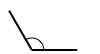
\includegraphics[scale=\shrinkfactor]{figures/30e6d029e2da9ba1853a868eb2f393092111abdd.png}



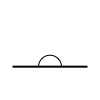
\includegraphics[scale=\shrinkfactor]{figures/567e8914a4f3bc1f9bca20b50f74d304dad89471.png}


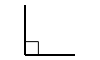
\includegraphics[scale=\shrinkfactor]{figures/07bf5a33ab5404dda360187045fc484bafcf6406.png}

\fbox{ 
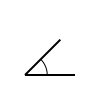
\includegraphics[scale=\shrinkfactor]{figures/37b74bb65d68f46dddef91f4180de8fb56af2027.png}

}

 

\paragraph{Hint 1}We can most easily identify a $90^\circ$ angle.  It looks like the corner of a rectangular piece of paper or a door.  


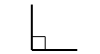
\includegraphics[scale=\shrinkfactor]{figures/59dcaf7caad1b34a49fc6b67de97830d5c26786c.png}

The $45^\circ$ angle will have to be smaller than that one.

\paragraph{Hint 2}A $45^\circ$ angle is $\frac{1}{2}$ the size of a $90^\circ$ angle.  

It takes two $45^\circ$ angles sitting side by side to make one $90^\circ$ angle.  Which angle could you fit $2$ times inside of a $90^\circ$ angle?

\paragraph{Hint 3}Here is a $90^\circ$ angle cut into $2$ angles of $45^\circ$.  

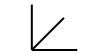
\includegraphics[scale=\shrinkfactor]{figures/917cdac7d04f1aaf0d4ee0269b2762d198ef3a3c.png}

\paragraph{Hint 4}The smallest angle pictured is a $45^\circ$ angle.  

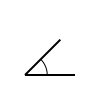
\includegraphics[scale=\shrinkfactor]{figures/37b74bb65d68f46dddef91f4180de8fb56af2027.png}



\medskip
\noindent
\textbf{Tags:} {\footnotesize CC.4.MD.C.5, SB.4.1.K.4.SR, Benchmark angles.1, Benchmark angles}\\
\textbf{Version:} 4cdbd1dc.. 2013-10-11
\smallskip\hrule





\section{\href{https://www.khanacademy.org/devadmin/content/items/x1caa681bcef7634e}{x1caa681bcef7634e}}

\noindent
**What is the measure of this angle?**


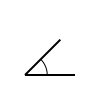
\includegraphics[scale=\shrinkfactor]{figures/37b74bb65d68f46dddef91f4180de8fb56af2027.png}

\paragraph{Ans} 

\fbox{ $45^\circ$

}

 $90^\circ$

$180^\circ$

$135^\circ$



\paragraph{Hint 1}We can most easily identify a $90^\circ$ angle.  It looks like the corner of a rectangular piece of paper or a door.  Does the angle in this problem look square like a $90^\circ$ angle?

\paragraph{Hint 2}A $180^\circ$ angle is twice the size of a $90^\circ$ angle.  It is called a *straight angle* and happens when one side of the angle rotates around to point in the opposite direction of the other side.  It looks like this:  

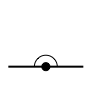
\includegraphics[scale=\shrinkfactor]{figures/856ba495997333078ad59534e55d1f3e88fb863f.png}

\paragraph{Hint 3}A $135^\circ$ angle is bigger than a $90^\circ$ angle and smaller than a $180^\circ$ angle.  Does the angle we are working on look bigger than $90^\circ$?

\paragraph{Hint 4}A $45^\circ$ angle is half the size of a $90^\circ$ angle.  Does the angle shown look like we could fit $2$ of them side by side in a $90^\circ$ angle?

\paragraph{Hint 5}The measure of the angle is $45^\circ$.



\medskip
\noindent
\textbf{Tags:} {\footnotesize CC.4.MD.C.5, SB.4.1.K.4.SR, Benchmark angles.2, Benchmark angles}\\
\textbf{Version:} 81b88e7a.. 2013-10-12
\smallskip\hrule





\section{\href{https://www.khanacademy.org/devadmin/content/items/x50309d5f1b142ab0}{x50309d5f1b142ab0}}

\noindent
**What is the measure of this angle?**


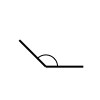
\includegraphics[scale=\shrinkfactor]{figures/3b29cb7bd47c46eb2ecd140dd305d1123b9185e6.png}

\paragraph{Ans} 

$45^\circ$

$90^\circ$

$180^\circ$

\fbox{ $135^\circ$

}

 

\paragraph{Hint 1}We can easily identify a $90^\circ$ angle.  It looks like the corner of a rectangular piece of paper or a door.  Does the angle in this problem look square like a $90^\circ$ angle?

\paragraph{Hint 2}A $180^\circ$ angle is twice the size of a $90^\circ$ angle.  It is called a *straight angle* and happens when one side of the angle rotates around to point in the opposite direction of the other side.  It looks like this:  

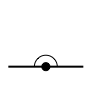
\includegraphics[scale=\shrinkfactor]{figures/856ba495997333078ad59534e55d1f3e88fb863f.png}

\paragraph{Hint 3}A $45^\circ$ angle is acute, which means that it is smaller than a $90^\circ$ angle.  Does the angle shown look smaller than $90^\circ$?

\paragraph{Hint 4}A $135^\circ$ angle is bigger than a $90^\circ$ angle and smaller than a $180^\circ$ angle.  Does the angle we are working on look bigger than $90^\circ$ and smaller than $180^\circ$?

\paragraph{Hint 5}The measure of the angle is $135^\circ$.



\medskip
\noindent
\textbf{Tags:} {\footnotesize CC.4.MD.C.5, SB.4.1.K.4.SR, Benchmark angles.2, Benchmark angles}\\
\textbf{Version:} c7b28af1.. 2013-10-12
\smallskip\hrule





\section{\href{https://www.khanacademy.org/devadmin/content/items/x6d37865e43597476}{x6d37865e43597476}}

\noindent
**What is the measure of this angle?**


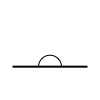
\includegraphics[scale=\shrinkfactor]{figures/567e8914a4f3bc1f9bca20b50f74d304dad89471.png}

\paragraph{Ans} 

$60^\circ$

$90^\circ$

\fbox{ $180^\circ$

}

 $120^\circ$



\paragraph{Hint 1}We can easily identify a $90^\circ$ angle.  It looks like the corner of a rectangular piece of paper or a door.  Does the angle in this problem look square like a $90^\circ$ angle?

\paragraph{Hint 2}A $60^\circ$ angle is acute, which means that it is smaller than a $90^\circ$ angle.  Does the angle shown look smaller than $90^\circ$?

\paragraph{Hint 3}A $180^\circ$ angle is twice the size of a $90^\circ$ angle.  It is called a *straight angle* and happens when one side of the angle rotates around to point in the opposite direction of the other side.  It looks like this:  

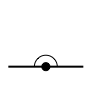
\includegraphics[scale=\shrinkfactor]{figures/856ba495997333078ad59534e55d1f3e88fb863f.png}

\paragraph{Hint 4}The measure of the angle is $180^\circ$.



\medskip
\noindent
\textbf{Tags:} {\footnotesize CC.4.MD.C.5, SB.4.1.K.4.SR, Benchmark angles.2, Benchmark angles}\\
\textbf{Version:} 9df90499.. 2013-10-12
\smallskip\hrule





\section{\href{https://www.khanacademy.org/devadmin/content/items/x8d5c6bc320e53991}{x8d5c6bc320e53991}}

\noindent
**What is the measure of this angle?**


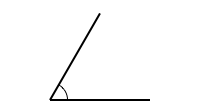
\includegraphics[scale=\shrinkfactor]{figures/0ab5a53f89e5f9dc3f4d81263d2c192ff74a873f.png}

\paragraph{Ans} 

\fbox{ $60^\circ$

}

 $90^\circ$

$120^\circ$

$180^\circ$



\paragraph{Hint 1}We can most easily identify a $90^\circ$ angle.  It looks like the corner of a rectangular piece of paper or a door.  Does the angle in this problem look square like a $90^\circ$ angle?

\paragraph{Hint 2}A $180^\circ$ angle is twice the size of a $90^\circ$ angle.  It is called a *straight angle* and happens when one side of the angle rotates around to point in the opposite direction of the other side.  It looks like this:  

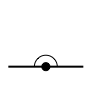
\includegraphics[scale=\shrinkfactor]{figures/856ba495997333078ad59534e55d1f3e88fb863f.png}

\paragraph{Hint 3}A $120^\circ$ angle is bigger than a $90^\circ$ angle and smaller than a $180^\circ$ angle.  Does the angle we are working on look bigger than $90^\circ$?

\paragraph{Hint 4}A $60^\circ$ angle is smaller than a $90^\circ$ angle.  Does the angle we are working on look smaller than $90^\circ$?

\paragraph{Hint 5}The measure of the angle is $60^\circ$.



\medskip
\noindent
\textbf{Tags:} {\footnotesize CC.4.MD.C.5, SB.4.1.K.4.SR, Benchmark angles.2, Benchmark angles}\\
\textbf{Version:} 4e1d1f6d.. 2013-10-12
\smallskip\hrule





\section{\href{https://www.khanacademy.org/devadmin/content/items/xb0afbe833bec4b15}{xb0afbe833bec4b15}}

\noindent
**What is the measure of this angle?**


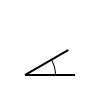
\includegraphics[scale=\shrinkfactor]{figures/d3a2a4fb2274b18d8b340c80127ae99c1ed8b1f9.png}

\paragraph{Ans} 

\fbox{ $30^\circ$

}

 $90^\circ$

$180^\circ$

$135^\circ$



\paragraph{Hint 1}We can most easily identify a $90^\circ$ angle.  It looks like the corner of a rectangular piece of paper or a door.  Does the angle in this problem look square like a $90^\circ$ angle?

\paragraph{Hint 2}A $180^\circ$ angle is twice the size of a $90^\circ$ angle.  It is called a *straight angle* and happens when one side of the angle rotates around to point in the opposite direction of the other side.  It looks like this:  

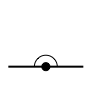
\includegraphics[scale=\shrinkfactor]{figures/856ba495997333078ad59534e55d1f3e88fb863f.png}

\paragraph{Hint 3}A $135^\circ$ angle is bigger than a $90^\circ$ angle and smaller than a $180^\circ$ angle.  Does the angle we are working on look bigger than $90^\circ$?

\paragraph{Hint 4}A $30^\circ$ angle is smaller than a $90^\circ$ angle.  Does the angle we are working on look smaller than $90^\circ$?

\paragraph{Hint 5}The measure of the angle is $30^\circ$.



\medskip
\noindent
\textbf{Tags:} {\footnotesize CC.4.MD.C.5, SB.4.1.K.4.SR, Benchmark angles.2, Benchmark angles}\\
\textbf{Version:} 19bd21e5.. 2013-10-12
\smallskip\hrule





\section{\href{https://www.khanacademy.org/devadmin/content/items/xedbfd6a3412204b7}{xedbfd6a3412204b7}}

\noindent
**What is the measure of this angle?**


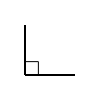
\includegraphics[scale=\shrinkfactor]{figures/e6ad77b54552295693aae7e39624ed456b552099.png}

\paragraph{Ans} 

$45^\circ$

\fbox{ $90^\circ$

}

 $180^\circ$

$135^\circ$



\paragraph{Hint 1}We can easily identify a $90^\circ$ angle.  It looks like the corner of a rectangular piece of paper or a door.  Does the angle in this problem look square like a $90^\circ$ angle?

\paragraph{Hint 2}We often see a square marking on $90^\circ$ angles to indicate that they are right angles.  When we see this, we can assume that the measure of the angle is $90^\circ$.

\paragraph{Hint 3}The measure of the angle is $90^\circ$.



\medskip
\noindent
\textbf{Tags:} {\footnotesize CC.4.MD.C.5, SB.4.1.K.4.SR, Benchmark angles.2, Benchmark angles}\\
\textbf{Version:} bfc6cd35.. 2013-10-12
\smallskip\hrule





\section{\href{https://www.khanacademy.org/devadmin/content/items/x5c354d48e3db6ac9}{x5c354d48e3db6ac9}}

\noindent
**Match these angles with their measures.**

There should be one angle in each category.

[[? categorization 1]]



\paragraph{Ans} Drag the cards to the correct categories. 

\paragraph{Hint 1}Let's arrange the angles from smallest to largest. 

\paragraph{Hint 2}The smallest angle is $30^\circ$, next is $90^\circ$, next is $135^\circ$, and the largest is $180^\circ$.

\paragraph{Hint 3}$30^\circ$ | $90^\circ$ | $135^\circ$ | $180^\circ$
:-: | :-: | :-: | :-:

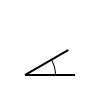
\includegraphics[scale=\shrinkfactor]{figures/d3a2a4fb2274b18d8b340c80127ae99c1ed8b1f9.png} | 
\includegraphics[scale=\shrinkfactor]{figures/e6ad77b54552295693aae7e39624ed456b552099.png} | 
\includegraphics[scale=\shrinkfactor]{figures/3b29cb7bd47c46eb2ecd140dd305d1123b9185e6.png} | 
\includegraphics[scale=\shrinkfactor]{figures/567e8914a4f3bc1f9bca20b50f74d304dad89471.png}



\medskip
\noindent
\textbf{Tags:} {\footnotesize CC.4.MD.C.5, SB.4.1.K.4.SR, Benchmark angles.3, Benchmark angles}\\
\textbf{Version:} ebe4f0d6.. 2013-10-12
\smallskip\hrule





\section{\href{https://www.khanacademy.org/devadmin/content/items/x8d85ca9ed1137ab4}{x8d85ca9ed1137ab4}}

\noindent
**Match these angles with their measures.**

There should be one angle in each category.

[[? categorization 1]]



\paragraph{Ans} Drag the cards to the correct categories. 

\paragraph{Hint 1}Let's arrange the angles from smallest to largest. 

\paragraph{Hint 2}The smallest angle is $30^\circ$, next is $60^\circ$, next is $90^\circ$, and the largest is $135^\circ$.

\paragraph{Hint 3}$30^\circ$ | $60^\circ$ | $90^\circ$ | $135^\circ$
:-: | :-: | :-: | :-:

\includegraphics[scale=\shrinkfactor]{figures/d3a2a4fb2274b18d8b340c80127ae99c1ed8b1f9.png} | 
\includegraphics[scale=\shrinkfactor]{figures/a78f141720cba4a3b167228345493573d23a2d23.png} | 
\includegraphics[scale=\shrinkfactor]{figures/e6ad77b54552295693aae7e39624ed456b552099.png} | 
\includegraphics[scale=\shrinkfactor]{figures/3b29cb7bd47c46eb2ecd140dd305d1123b9185e6.png}



\medskip
\noindent
\textbf{Tags:} {\footnotesize CC.4.MD.C.5, SB.4.1.K.4.SR, Benchmark angles.3, Benchmark angles}\\
\textbf{Version:} 7a74a7fd.. 2013-10-12
\smallskip\hrule





\section{\href{https://www.khanacademy.org/devadmin/content/items/x90132d401d6471d6}{x90132d401d6471d6}}

\noindent
**Match these angles with their measures.**

There should be one angle in each category.

[[? categorization 1]]



\paragraph{Ans} Drag the cards to the correct categories. 

\paragraph{Hint 1}Let's arrange the angles from smallest to largest. 

\paragraph{Hint 2}The smallest angle is $45^\circ$, next is $90^\circ$, next is $135^\circ$, and the largest is $180^\circ$.

\paragraph{Hint 3}$45^\circ$ | $90^\circ$ | $135^\circ$ | $180^\circ$
:-: | :-: | :-: | :-:

\includegraphics[scale=\shrinkfactor]{figures/37b74bb65d68f46dddef91f4180de8fb56af2027.png} | 
\includegraphics[scale=\shrinkfactor]{figures/e6ad77b54552295693aae7e39624ed456b552099.png} | 
\includegraphics[scale=\shrinkfactor]{figures/3b29cb7bd47c46eb2ecd140dd305d1123b9185e6.png} | 
\includegraphics[scale=\shrinkfactor]{figures/567e8914a4f3bc1f9bca20b50f74d304dad89471.png}



\medskip
\noindent
\textbf{Tags:} {\footnotesize CC.4.MD.C.5, SB.4.1.K.4.SR, Benchmark angles.3, Benchmark angles}\\
\textbf{Version:} aae56960.. 2013-10-12
\smallskip\hrule





\section{\href{https://www.khanacademy.org/devadmin/content/items/xd5177ccaf78d3a30}{xd5177ccaf78d3a30}}

\noindent
**Match these angles with their measures.**

There should be one angle in each category.

[[? categorization 1]]



\paragraph{Ans} Drag the cards to the correct categories. 

\paragraph{Hint 1}Let's arrange the angles from smallest to largest. 

\paragraph{Hint 2}The smallest angle is $30^\circ$, next is $45^\circ$, next is $60^\circ$, and the largest is $90^\circ$.

\paragraph{Hint 3}$30^\circ$ | $45^\circ$ | $60^\circ$ | $90^\circ$
:-: | :-: | :-: | :-:

\includegraphics[scale=\shrinkfactor]{figures/d3a2a4fb2274b18d8b340c80127ae99c1ed8b1f9.png} | 
\includegraphics[scale=\shrinkfactor]{figures/37b74bb65d68f46dddef91f4180de8fb56af2027.png} | 
\includegraphics[scale=\shrinkfactor]{figures/a78f141720cba4a3b167228345493573d23a2d23.png} | 
\includegraphics[scale=\shrinkfactor]{figures/e6ad77b54552295693aae7e39624ed456b552099.png}



\medskip
\noindent
\textbf{Tags:} {\footnotesize CC.4.MD.C.5, SB.4.1.K.4.SR, Benchmark angles.3, Benchmark angles}\\
\textbf{Version:} c68ca331.. 2013-10-12
\smallskip\hrule





\section{\href{https://www.khanacademy.org/devadmin/content/items/xe5974944cc434f58}{xe5974944cc434f58}}

\noindent
**Match these angles with their measures.**

There should be one angle in each category.

[[? categorization 1]]



\paragraph{Ans} Drag the cards to the correct categories. 

\paragraph{Hint 1}Let's arrange the angles from smallest to largest. 

\paragraph{Hint 2}The smallest angle is $30^\circ$, next is $60^\circ$, next is $90^\circ$, and the largest is $135^\circ$.

\paragraph{Hint 3}$30^\circ$ | $60^\circ$ | $90^\circ$ | $135^\circ$
:-: | :-: | :-: | :-:

\includegraphics[scale=\shrinkfactor]{figures/d3a2a4fb2274b18d8b340c80127ae99c1ed8b1f9.png}  | 
\includegraphics[scale=\shrinkfactor]{figures/a78f141720cba4a3b167228345493573d23a2d23.png} | 
\includegraphics[scale=\shrinkfactor]{figures/e6ad77b54552295693aae7e39624ed456b552099.png} | 
\includegraphics[scale=\shrinkfactor]{figures/3b29cb7bd47c46eb2ecd140dd305d1123b9185e6.png}



\medskip
\noindent
\textbf{Tags:} {\footnotesize CC.4.MD.C.5, SB.4.1.K.4.SR, Benchmark angles.3, Benchmark angles}\\
\textbf{Version:} 91c7a197.. 2013-10-12
\smallskip\hrule





\section{\href{https://www.khanacademy.org/devadmin/content/items/xfc1619c4ab461ddb}{xfc1619c4ab461ddb}}

\noindent
**Match these angles with their measures.**

There should be one angle in each category.

[[? categorization 1]]



\paragraph{Ans} Drag the cards to the correct categories. 

\paragraph{Hint 1}Let's arrange the angles from smallest to largest. 

\paragraph{Hint 2}The smallest angle is $30^\circ$, next is $60^\circ$, next is $90^\circ$, and the largest is $180^\circ$.

\paragraph{Hint 3}$30^\circ$ | $60^\circ$ | $90^\circ$ | $180^\circ$
:-: | :-: | :-: | :-:

\includegraphics[scale=\shrinkfactor]{figures/d3a2a4fb2274b18d8b340c80127ae99c1ed8b1f9.png} | 
\includegraphics[scale=\shrinkfactor]{figures/a78f141720cba4a3b167228345493573d23a2d23.png} | 
\includegraphics[scale=\shrinkfactor]{figures/e6ad77b54552295693aae7e39624ed456b552099.png} | 
\includegraphics[scale=\shrinkfactor]{figures/567e8914a4f3bc1f9bca20b50f74d304dad89471.png}



\medskip
\noindent
\textbf{Tags:} {\footnotesize CC.4.MD.C.5, SB.4.1.K.4.SR, Benchmark angles.3, Benchmark angles}\\
\textbf{Version:} 5fa7f6a4.. 2013-10-12
\smallskip\hrule





\section{\href{https://www.khanacademy.org/devadmin/content/items/x29ff9407ced34f2c}{x29ff9407ced34f2c}}

\noindent
All of these shapes are *regular*, meaning that all of the sides of each shape are the same length.

**Which of these regular shapes has $60^\circ$ angles between its sides?**



\paragraph{Ans} 


\includegraphics[scale=\shrinkfactor]{figures/498a6b09730fdba2360826c138eeee142e8cccc1.png}

\fbox{ 
\includegraphics[scale=\shrinkfactor]{figures/bd0208484f0985a689654e9316bcaeff83c10bc5.png}

}

 
\includegraphics[scale=\shrinkfactor]{figures/7d98a99c75a84da8f748444ad7a3a8053be16a27.png}



\paragraph{Hint 1}This regular pentagon has $5$ obtuse angles (larger than $90^\circ$).  If you are not sure, hold up the corner of a rectangular piece of paper to each angle and compare each to the $90^\circ$ angle of the paper.


\includegraphics[scale=\shrinkfactor]{figures/498a6b09730fdba2360826c138eeee142e8cccc1.png}

\paragraph{Hint 2}This regular octagon has $8$ obtuse angles (larger than $90^\circ$).  If you are not sure, hold up the corner of a rectangular piece of paper to each angle and compare each to the $90^\circ$ angle of the paper.


\includegraphics[scale=\shrinkfactor]{figures/7d98a99c75a84da8f748444ad7a3a8053be16a27.png}

\paragraph{Hint 3}This equilateral triangle has $3$ angles which are all equal to $60^\circ$.


\includegraphics[scale=\shrinkfactor]{figures/bd0208484f0985a689654e9316bcaeff83c10bc5.png}



\medskip
\noindent
\textbf{Tags:} {\footnotesize CC.4.MD.C.5, SB.4.1.K.4.SR, Benchmark angles.4, Benchmark angles}\\
\textbf{Version:} 373ed1ec.. 2013-10-15
\smallskip\hrule





\section{\href{https://www.khanacademy.org/devadmin/content/items/x6cff27b8821951af}{x6cff27b8821951af}}

\noindent
This triangle has angle measures of $30^\circ$ and $120^\circ$.  

**Identify which angle or angles in the triangle has each angle measure.**


\includegraphics[scale=\shrinkfactor]{figures/b9f5003c0001dcfb9fb4d1e61e8b8d7445cf9e8c.png}

[[? categorization 1]]

\paragraph{Ans} Drag the angle names to the correct measurement. 

\paragraph{Hint 1}This triangle has $2$ small angles, and $1$ larger angle.

\paragraph{Hint 2}The small angles are $\angle B$ and $\angle C$.  The larger angle is $\angle A$.

\paragraph{Hint 3}The measures of the angles are:  
$\angle A=120^\circ$  
$\angle B=30^\circ$  
$\angle C=30^\circ$



\medskip
\noindent
\textbf{Tags:} {\footnotesize CC.4.MD.C.5, SB.4.1.K.4.SR, Benchmark angles.4, Benchmark angles}\\
\textbf{Version:} c3fdb3ac.. 2013-10-12
\smallskip\hrule





\section{\href{https://www.khanacademy.org/devadmin/content/items/xd46610fd6b543fcd}{xd46610fd6b543fcd}}

\noindent
**Which of these triangles has a $90^\circ$ angle?**



\paragraph{Ans} 


\includegraphics[scale=\shrinkfactor]{figures/ee7f87a00acb47dec4f2b2eed9a6741b21afc47d.png}


\includegraphics[scale=\shrinkfactor]{figures/2d844a51b839d81f30ea0fd7869869c78159abd0.png}

\fbox{ 
\includegraphics[scale=\shrinkfactor]{figures/0cd19d8e042c76c262a5054d4fdc63823c75ae58.png}

}

 

\paragraph{Hint 1}This triangle has $3$ acute angles, all smaller than $90^\circ$.  If you are not sure, hold up the corner of a rectangular piece of paper to each angle and compare each to the $90^\circ$ angle of the paper.


\includegraphics[scale=\shrinkfactor]{figures/ee7f87a00acb47dec4f2b2eed9a6741b21afc47d.png}

\paragraph{Hint 2}This triangle has $1$ obtuse angle, larger than $90^\circ$, and $2$ acute angles, smaller than $90^\circ$.  If you are not sure, hold up the corner of a rectangular piece of paper to each angle and compare.


\includegraphics[scale=\shrinkfactor]{figures/2d844a51b839d81f30ea0fd7869869c78159abd0.png}

\paragraph{Hint 3}This triangle has $1$ right angle, equal to $90^\circ$.  If you are not sure, hold up the corner of a rectangular piece of paper to the largest angle and compare.


\includegraphics[scale=\shrinkfactor]{figures/0cd19d8e042c76c262a5054d4fdc63823c75ae58.png}



\medskip
\noindent
\textbf{Tags:} {\footnotesize CC.4.MD.C.5, SB.4.1.K.4.SR, Benchmark angles.4, Benchmark angles}\\
\textbf{Version:} 3bbb9a8c.. 2013-10-15
\smallskip\hrule





\section{\href{https://www.khanacademy.org/devadmin/content/items/xef45230d848911b2}{xef45230d848911b2}}

\noindent
All of these shapes are *regular*, meaning that all of the sides of each shape are the same length.

**Which of these regular shapes has $60^\circ$ angles between its sides?**



\paragraph{Ans} 


\includegraphics[scale=\shrinkfactor]{figures/0245164f3f4897772e76d361f955075a80732b03.png}

\fbox{ 
\includegraphics[scale=\shrinkfactor]{figures/bd0208484f0985a689654e9316bcaeff83c10bc5.png}

}

 
\includegraphics[scale=\shrinkfactor]{figures/2ab3724280597cbfc2e5a5a20f466cee45636a9f.png}



\paragraph{Hint 1}This regular hexagon has $6$ obtuse angles (larger than $90^\circ$).  If you are not sure, hold up the corner of a rectangular piece of paper to each angle and compare each to the $90^\circ$ angle of the paper.


\includegraphics[scale=\shrinkfactor]{figures/0245164f3f4897772e76d361f955075a80732b03.png}

\paragraph{Hint 2}This square has $4$ right angles (equal to $90^\circ$).  If you are not sure, hold up the corner of a rectangular piece of paper to each angle and compare each to the $90^\circ$ angle of the paper.


\includegraphics[scale=\shrinkfactor]{figures/2ab3724280597cbfc2e5a5a20f466cee45636a9f.png}

\paragraph{Hint 3}This equilateral triangle has $3$ angles which are all equal to $60^\circ$.


\includegraphics[scale=\shrinkfactor]{figures/bd0208484f0985a689654e9316bcaeff83c10bc5.png}



\medskip
\noindent
\textbf{Tags:} {\footnotesize CC.4.MD.C.5, SB.4.1.K.4.SR, Benchmark angles.4, Benchmark angles}\\
\textbf{Version:} de638271.. 2013-10-15
\smallskip\hrule





\section{\href{https://www.khanacademy.org/devadmin/content/items/xf56c85092c5059c0}{xf56c85092c5059c0}}

\noindent
This triangle has angle measures of $45^\circ$ and $90^\circ$.  

**Identify which angle or angles in the triangle has each angle measure.**


\includegraphics[scale=\shrinkfactor]{figures/80d671a94d27cf5e42ef86661ca8f847863726f1.png}

[[? categorization 1]]

\paragraph{Ans} Drag the angle names to the correct measurement. 

\paragraph{Hint 1}This triangle has $2$ small angles, and $1$ larger angle.

\paragraph{Hint 2}The small angles are $\angle A$ and $\angle C$.  The larger angle is $\angle B$.

\paragraph{Hint 3}The measures of the angles are:  
$\angle A=45^\circ$  
$\angle B=90^\circ$  
$\angle C=45^\circ$



\medskip
\noindent
\textbf{Tags:} {\footnotesize CC.4.MD.C.5, SB.4.1.K.4.SR, Benchmark angles.4, Benchmark angles}\\
\textbf{Version:} c97ba279.. 2013-10-12
\smallskip\hrule





\section{\href{https://www.khanacademy.org/devadmin/content/items/xfc906b64a303a11f}{xfc906b64a303a11f}}

\noindent
This triangle has angle measures of $30^\circ$, $60^\circ$, and $90^\circ$.  

**Identify which angle in the triangle has each angle measure.**

There should be one angle in each category.


\includegraphics[scale=\shrinkfactor]{figures/76b085ab1f9ed7cbf048cd93cdeccd8aebffd0f2.png}

[[? categorization 1]]

\paragraph{Ans} Drag the angle names to the correct measurement. 

\paragraph{Hint 1}We can think about the order of the angles from smallest to largest.  

The smallest angle in any triangle is across from the shortest side.  The largest angle is across from the longest side.

\paragraph{Hint 2}The smallest angle is $\angle B$, next is $\angle C$, and the largest is $\angle A$.

\paragraph{Hint 3}The measures of the angles are:  
$\angle B=30^\circ$  
$\angle C=60^\circ$  
$\angle A=90^\circ$



\medskip
\noindent
\textbf{Tags:} {\footnotesize CC.4.MD.C.5, SB.4.1.K.4.SR, Benchmark angles.4, Benchmark angles}\\
\textbf{Version:} 7ad8a273.. 2013-10-12
\smallskip\hrule





\section{\href{https://www.khanacademy.org/devadmin/content/items/x2af6283782953afa}{x2af6283782953afa}}

\noindent
**Match these angles with the closest measure.**

There may be more than one card in each category.

[[? categorization 1]]


\paragraph{Ans} Drag the cards to the correct categories. 

\paragraph{Hint 1}When a pair of scissors is closed, the angle between the blades is $0^\circ$.

\paragraph{Hint 2}When a person is sitting up straight in a chair, his legs and back make a $90^\circ$ angle.

A ladder going up to a diving board makes a $90^\circ$ angle with the diving board.

\paragraph{Hint 3}When a person is lying down flat, his legs and back make a *straight angle* of $180^\circ$.

\paragraph{Hint 4}$0^\circ$  

* The blades of a pair of scissors when closed

$90^\circ$ 
 
* A person's legs and back when sitting up straight in a chair
* A diving board and the ladder going up to it


$180^\circ$  

* A person's legs and back when lying down flat




\medskip
\noindent
\textbf{Tags:} {\footnotesize Image needs attribution, CC.4.MD.C.5, SB.4.1.K.4.SR, Benchmark angles.5, Benchmark angles}\\
\textbf{Version:} 2c63efb6.. 2013-10-15
\smallskip\hrule





\section{\href{https://www.khanacademy.org/devadmin/content/items/x4a41ed86b953d410}{x4a41ed86b953d410}}

\noindent
**Match these angles with the closest measure.**

There may be more than one card in each category.

[[? categorization 1]]


\paragraph{Ans} Drag the cards to the correct categories. 

\paragraph{Hint 1}When a pair of scissors is closed, the angle between the blades is $0^\circ$.

\paragraph{Hint 2}When a person is sitting up straight in a chair, his legs and back make a $90^\circ$ angle.

A ladder going up to a diving board makes a $90^\circ$ angle with the diving board.

\paragraph{Hint 3}When a person is lying down flat, his legs and back make a *straight angle* of $180^\circ$.

\paragraph{Hint 4}$0^\circ$  

* The blades of a pair of scissors when closed

$90^\circ$ 
 
* A person's legs and back when sitting up straight in a chair
* A diving board and the ladder going up to it


$180^\circ$  

* A person's legs and back when lying down flat




\medskip
\noindent
\textbf{Tags:} {\footnotesize Image needs attribution, CC.4.MD.C.5, SB.4.1.K.4.SR, Benchmark angles.5, Benchmark angles}\\
\textbf{Version:} 6730ec4a.. 2013-10-15
\smallskip\hrule





\section{\href{https://www.khanacademy.org/devadmin/content/items/x615a6e4f048a23b0}{x615a6e4f048a23b0}}

\noindent
**Match these angles with their measures.**

There may be more than one card in each category.

[[? categorization 1]]


\paragraph{Ans} Drag the cards to the correct categories. 

\paragraph{Hint 1}When a crocodile's mouth is closed, the angle between its jaws is $0^\circ$.

\paragraph{Hint 2}A capital letter L in block printing forms a $90^\circ$ angle.

\paragraph{Hint 3}When a book is open all the way flat on a table, the covers make a *straight angle* of $180^\circ$.

When you turn to face the opposite direction, you make a $180^\circ$ turn.

\paragraph{Hint 4}$0^\circ$  

* A crocodile's mouth when it is closed

$90^\circ$ 
 
* A capital letter L in block printing

$180^\circ$  

* The front and back cover of a book that is open all the way flat on the table  
* The angle you turn to face the opposite direction



\medskip
\noindent
\textbf{Tags:} {\footnotesize Image needs attribution, CC.4.MD.C.5, SB.4.1.K.4.SR, Benchmark angles.5, Benchmark angles}\\
\textbf{Version:} bafba8d3.. 2013-10-15
\smallskip\hrule





\section{\href{https://www.khanacademy.org/devadmin/content/items/x64de888209ceabe2}{x64de888209ceabe2}}

\noindent
**Match these angles with the closest measure.**

There may be more than one card in each category.

[[? categorization 1]]


\paragraph{Ans} Drag the cards to the correct categories. 

\paragraph{Hint 1}At $12$:$00$, the angle between the hands of a clock is $0^\circ$.

\paragraph{Hint 2}The answers going *across* on a crossword puzzle are at an angle of $90^\circ$ from the answers going *down*.

\paragraph{Hint 3}At $8$:$00$, the angle between the hands of a clock is $120^\circ$.  You can think of it as covering $\frac{1}{3}$ of the total $360^\circ$ of the circle.

We can be sure that the sides of a regular hexagon are not at an angle of $0^\circ$.  Because the cells of the honeycomb are not squares or rectangles, they do not have angles measuring $90^\circ$.  The angles of a regular hexagon are $120^\circ$.

\paragraph{Hint 4}$0^\circ$  

* The angle of the hands on a clock at $12$:$00$

$90^\circ$ 
 
* The angle between the "Across" answers and the "Down" answers on a crossword puzzle grid

$120^\circ$  

* The angle of the hands on a clock at $8$:$00$
* The angles of the sides of one hexagonal cell in a honeycomb




\medskip
\noindent
\textbf{Tags:} {\footnotesize Image needs attribution, CC.4.MD.C.5, SB.4.1.K.4.SR, Benchmark angles.5, Benchmark angles}\\
\textbf{Version:} 8530e71f.. 2013-10-15
\smallskip\hrule





\section{\href{https://www.khanacademy.org/devadmin/content/items/xb4d725629a955ae4}{xb4d725629a955ae4}}

\noindent
**Match these angles with the closest measure.**

There may be more than one card in each category.

[[? categorization 1]]


\paragraph{Ans} Drag the cards to the correct categories. 

\paragraph{Hint 1}When a shark's mouth is closed, the angle between its jaws is $0^\circ$.

\paragraph{Hint 2}At $4$:$30$, the hands on a clock are at a $45^\circ$ angle.  We can see that it is half of the $90^\circ$ angle between the $3$ and the $6$.

Two slices of an $8$-slice round pizza would make one quarter of the pizza, so they would make an angle of $90^\circ$.  One slice would make half of that angle, so it would be $45^\circ$.

\paragraph{Hint 3}A number $2$ on a digital watch is made up of $5$ segments.  Each one is at an angle of $90^\circ$ with the other adjacent segment or segments.

\paragraph{Hint 4}$0^\circ$  

* The jaws of a shark with its mouth closed

$45^\circ$ 
 
* The angle of the hands on a clock at $4$:$30$
* The point of a slice of an $8$-slice pizza


$90^\circ$  

* The angle between the line segments used to make a number $2$ on a digital watch




\medskip
\noindent
\textbf{Tags:} {\footnotesize Image needs attribution, CC.4.MD.C.5, SB.4.1.K.4.SR, Benchmark angles.5, Benchmark angles}\\
\textbf{Version:} 905b4001.. 2013-10-15
\smallskip\hrule





\section{\href{https://www.khanacademy.org/devadmin/content/items/xe2dda50d63e00f1c}{xe2dda50d63e00f1c}}

\noindent
**Match these angles with their measures.**

There may be more than one card in each category.

[[? categorization 1]]


\paragraph{Ans} Drag the cards to the correct categories. 

\paragraph{Hint 1}When a book is closed, the angle between the front and back covers is $0^\circ$.

When a book is open all the way flat on a table, the covers make a *straight angle* of $180^\circ$.

\paragraph{Hint 2}When a butterfly's wings are pointing up together, they are not rotated apart at all, so the angle between them is $0^\circ$.  

\includegraphics[scale=\shrinkfactor]{figures/bde4441a2a7d3232258295879ad1f4f45bc5b837.jpeg}

When a butterfly's wings are open all the way, they stretch out parallel to the ground and make an angle of $180^\circ$.  

\includegraphics[scale=\shrinkfactor]{figures/0a0d076d5698440c5014268d0af9d3e25b3230fc.jpeg}

When a butterfly's wings are open half way, each one makes an angle of $45^\circ$ from their straight-up position.  Together they make an angle of $90^\circ$.  

\includegraphics[scale=\shrinkfactor]{figures/0e6ca22c3d75533f11159c3a8a5a44d38957aa1a.jpeg}

\paragraph{Hint 3}$0^\circ$  

* The front and back cover of a book that is closed  
* A butterfly's wings when they are pointing up together

$90^\circ$  

* A butterfly's wings when they are halfway open

$180^\circ$  

* The front and back cover of a book that is open all the way flat on the table  
* A butterfly's wings when they are fully open and parallel to the ground



\medskip
\noindent
\textbf{Tags:} {\footnotesize Image needs attribution, CC.4.MD.C.5, SB.4.1.K.4.SR, Benchmark angles.5, Benchmark angles}\\
\textbf{Version:} 2c46653b.. 2013-10-15
\smallskip\hrule



%%  Create a directory called 'figures' in latex dir and run the following command 
%  wget -N \
%    https://ka-perseus-graphie.s3.amazonaws.com/30e6d029e2da9ba1853a868eb2f393092111abdd.png \
%    https://ka-perseus-graphie.s3.amazonaws.com/567e8914a4f3bc1f9bca20b50f74d304dad89471.png \
%    https://ka-perseus-graphie.s3.amazonaws.com/d3a2a4fb2274b18d8b340c80127ae99c1ed8b1f9.png \
%    https://ka-perseus-graphie.s3.amazonaws.com/e6ad77b54552295693aae7e39624ed456b552099.png \
%    https://ka-perseus-graphie.s3.amazonaws.com/59dcaf7caad1b34a49fc6b67de97830d5c26786c.png \
%    https://ka-perseus-graphie.s3.amazonaws.com/a78f141720cba4a3b167228345493573d23a2d23.png \
%    https://ka-perseus-graphie.s3.amazonaws.com/8eb18621606206c7adf43aa4f147027fdea82fad.png \
%    https://ka-perseus-graphie.s3.amazonaws.com/fabb944602f99b6fe0a5d55e7d841f87d0cbb415.png \
%    https://ka-perseus-graphie.s3.amazonaws.com/07bf5a33ab5404dda360187045fc484bafcf6406.png \
%    https://ka-perseus-graphie.s3.amazonaws.com/5a8d12cf1b68c217e145c1ab706ff0ac470bb360.png \
%    https://ka-perseus-graphie.s3.amazonaws.com/32e70b8ce2cad5546c56f4c5d1a1f283fdc91895.png \
%    https://ka-perseus-graphie.s3.amazonaws.com/37b74bb65d68f46dddef91f4180de8fb56af2027.png \
%    https://ka-perseus-graphie.s3.amazonaws.com/917cdac7d04f1aaf0d4ee0269b2762d198ef3a3c.png \
%    https://ka-perseus-graphie.s3.amazonaws.com/856ba495997333078ad59534e55d1f3e88fb863f.png \
%    https://ka-perseus-graphie.s3.amazonaws.com/3b29cb7bd47c46eb2ecd140dd305d1123b9185e6.png \
%    https://ka-perseus-graphie.s3.amazonaws.com/0ab5a53f89e5f9dc3f4d81263d2c192ff74a873f.png \
%    https://ka-perseus-graphie.s3.amazonaws.com/498a6b09730fdba2360826c138eeee142e8cccc1.png \
%    https://ka-perseus-graphie.s3.amazonaws.com/bd0208484f0985a689654e9316bcaeff83c10bc5.png \
%    https://ka-perseus-graphie.s3.amazonaws.com/7d98a99c75a84da8f748444ad7a3a8053be16a27.png \
%    https://ka-perseus-graphie.s3.amazonaws.com/b9f5003c0001dcfb9fb4d1e61e8b8d7445cf9e8c.png \
%    https://ka-perseus-graphie.s3.amazonaws.com/ee7f87a00acb47dec4f2b2eed9a6741b21afc47d.png \
%    https://ka-perseus-graphie.s3.amazonaws.com/2d844a51b839d81f30ea0fd7869869c78159abd0.png \
%    https://ka-perseus-graphie.s3.amazonaws.com/0cd19d8e042c76c262a5054d4fdc63823c75ae58.png \
%    https://ka-perseus-graphie.s3.amazonaws.com/0245164f3f4897772e76d361f955075a80732b03.png \
%    https://ka-perseus-graphie.s3.amazonaws.com/2ab3724280597cbfc2e5a5a20f466cee45636a9f.png \
%    https://ka-perseus-graphie.s3.amazonaws.com/80d671a94d27cf5e42ef86661ca8f847863726f1.png \
%    https://ka-perseus-graphie.s3.amazonaws.com/76b085ab1f9ed7cbf048cd93cdeccd8aebffd0f2.png \
%    https://ka-perseus-images.s3.amazonaws.com/bde4441a2a7d3232258295879ad1f4f45bc5b837.jpeg \
%    https://ka-perseus-images.s3.amazonaws.com/0a0d076d5698440c5014268d0af9d3e25b3230fc.jpeg \
%    https://ka-perseus-images.s3.amazonaws.com/0e6ca22c3d75533f11159c3a8a5a44d38957aa1a.jpeg \


\end{document}
